% ex: tw=74 ts=4 sw=4
\documentclass{article}
\usepackage[utf8]{inputenc}
\usepackage[normalem]{ulem}
\usepackage{xkeyval}
\usepackage[bookmarksnumbered]{hyperref}
%\hypersetup{pdfborder=0 0 0}
\usepackage{multirow}
\usepackage{todonotes}
\usepackage[english]{babel}
\usepackage{tabulary}
\usepackage{tabularx}
%\usepackage{fullpage}
%\usepackage{natbib}
\usepackage[all]{hypcap}
\usepackage{verbatim}
\usepackage{graphicx}
\usepackage{mathtools} %amsmath minus some quirks
%\usepackage[usenames,dvipsnames]{xcolor}
\usepackage{color}
%\usepackage{listings}
\usepackage{listingsutf8}
\usepackage{frame}
\usepackage{float}
\usepackage{verbatim}
\usepackage{cmap}
\usepackage{hyperref}
\usepackage{wrapfig}

\definecolor{gray}{rgb}{0.5,0.5,0.5}

%\newcommand{\comment}[1]{}
\newcommand{\wire}{\texttt}

\begin{document}

\lstset{breaklines=true,
	extendedchars=\true,
	inputencoding=utf8/latin1,
	title=\lstname,
	frame=shadowbox,
	rulesepcolor=\color{gray},
	tabsize=8,
	basicstyle=\footnotesize,
	numbers=left,                   % where to put the line-numbers
	numberstyle=\tiny\color{gray}}

% Title page.

\begin{titlepage}
\begin{center}
	{14:332:438 - Capstone Design, Digital Systems}
	{802.16-2009 OFDM PHY - Digital Realm Transmitter Implimentation}
	{Cody Schafer}
	{
		Submitted in partial fulfillment of the requirements for the \\
		Bachelor of Science Degree
	}
	{\today}
	{
		Electrical and Computer Engineering Dept. \\
		School of Engineering \\
		Rutgers University
	}
\end{center}
\end{titlepage}


\tableofcontents

% What is it, What are we doing, 

\section{Project Overview}
We are developing a minimal 802.16-2009 OFDM Transmitter PHY.  This PHY
supports only QPSK-1/2 modulation-convolution rate. Additionally, any
components not relevant to unlicensed bands are omitted.  All optional items
are omitted.

This PHY requires the cooperation of a MAC layer implementation which is
compliant with the 802.16-2009 standard in order for the compliance
expectations (\autoref{sec:comply}) to be met.

\begin{wrapfigure}{r}{0.5\textwidth}
\begin{center}
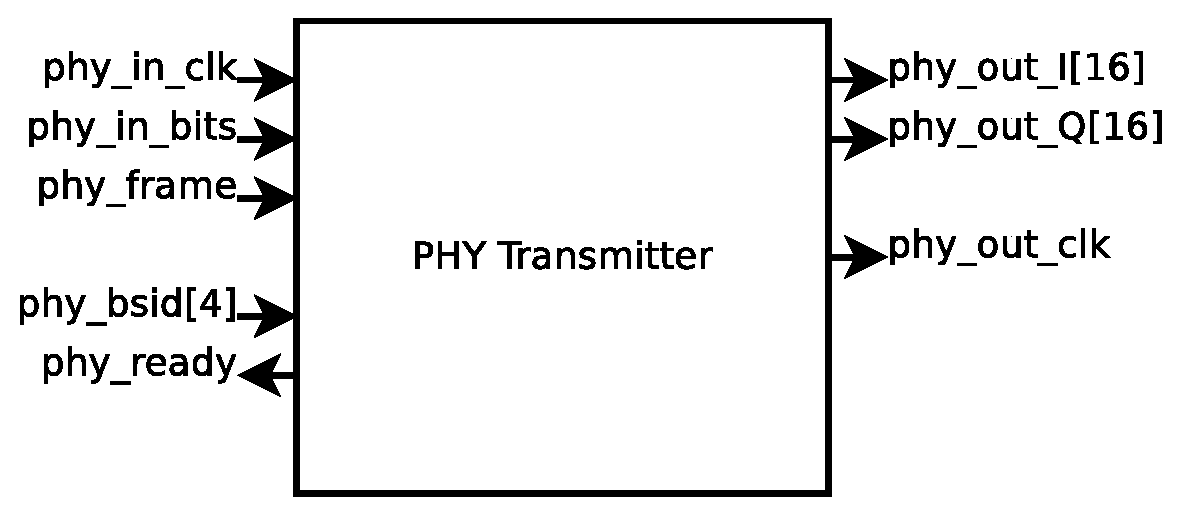
\includegraphics[width=0.48\textwidth]{t_block}
\caption{Overall Transmitter Interface}
\label{fiig:all-blockl}
\end{center}
\end{wrapfigure}

\begin{comment}
\todo[inline]{Derive the product from the needs}
\end{comment}

	\subsection{End Market Expectations}
	Currently IEEE 802.16, also known as ``WiMAX'', has seen little
	deployment in the United States and western Europe while being
	moderately deployed in Asian nations and Eastern European markets.
	To be useful in western areas, WiMAX has to effectively compete
	with both consumer owned Wifi hot-spots and the various cell phone
	networks. Given the impressively low cost of both cellular and Wifi
	(802.11) systems combined with the expectation that they work well
	in mobile devices, this physical layer (PHY) targets both
	simplicity (to reduce cost) and reduced power consumption.

	\subsection{Degree of standards compliance and scope limitations}
	\label{sec:comply}
	The 802.16 standard specifies multiple layers of a WiMAX device,
	including a ``Service-specific convergence
	sublayer''~\cite[section 5]{IEEE:802.16}, a MAC
	sublayer~\cite[section 6]{IEEE:802.16}, a Security
	sublayer~\cite[section 7]{IEEE:802.16}, and the Physical
	layer~\cite[section 8]{IEEE:802.16}. 
	
	The PHY, while being described within section 8 of the 802.16-2009
	document, is additionally subject to certain constraints and
	requirements stipulated within the other sections.  These sections
	where only utilized to the extent to which they apply to design of
	the PHY component.

	Applicable sections of \cite{IEEE:802.16}.
	\begin{itemize}
		\item Section 8.3 - OFDM description
		\item Section 8.3.3.4.1 - Data Modulation: implementation
			is not compliant with this section, only QPSK
			modulation is supported.
		\item 8.3.3.4.3 - Rate ID encodings: not compliant with
			this section, only the QPSK-1/2 rate ID is supported.
		\item 8.3.5.1.1 - DL subchannelization: Rate ID
	\end{itemize}

% Overarching design and spec items.
\section{OFDM Parameters}

\subsection{Primitive Parameters}

\begin{description}
	\item[BW]: This is the nominal channel bandwidth.
	\item[$N_{used}$]: Number of used subcarriers.
	\item[n]: Sampling factor. This parameter, in conjunction with BW
		and $N_{used}$ determines the subcarrier spacing, and the
		useful symbol time.
	\item[G]: This is the ratio of CP time to ``useful'' time.
\end{description}


%\todo[inline]{Insert a table of the values that are fixed by the standard and our implimentation limitations}

\subsection{Derived Parameters}

\begin{description}
	\item[$N_{FFT}$]: Smallest power of two greater than $N_{used}$
	\item[Sampling Frequency]: $F_s = floor ( n \cdot BW / 8000 )
		\times 8000 $
	\item[Subcarrier spacing]: $\Delta f = F s / N_{FFT} $
	\item[Useful symbol time]: $T_b = 1 / \Delta f$
	\item[CP Time]: $T_g = G \cdot T_b$
	\item[OFDM Symbol Time]: $T_s = T_b + T_g$
	\item[Sampling time]: $T_b / N_{FFT}$
\end{description}

% \todo[inline]{Tables of valid values for each of the derived values}

\section{External Interface to the PHY Transmitter}
\label{sec:frame}
The MAC interfaces with the PHY module by sending frames (with the
appropriate headers and padding included) as a stream of bits.  These bits
are clocked via the \textbf{mac\_clk\_in} line, and must only be sent when
the \textbf{mac\_sending\_frame} line is high.  The state of the
\textbf{mac\_sending\_frame} line must be low when not sending a frame, and
must be lowered and raised between frames that would otherwise be abutting.
The frequency of \textbf{mac\_clk\_in} must be less than or equal to half
of the \textbf{phy\_clock}.

The \textbf{phy\_ready} line is a signal to the mac that it is ready for a
new frame to be inputted, and should not be ignored.

The structure of individual frames detailed in section 8.3.5 of IEEE
802.16-2009.  Each frame contains a header, up to 4 DL sub-frames (each with
their own structure also defined in IEEE802.16-2009 section 8.3.5) and some
number of UL sub-frames.  Note that due to fixing certain implementation
parameters, some fields are constrained further than mentioned within the
standard.

\begin{description}
	\item[Frame Header - Rate\_ID] is fixed at '1' indicating CPS
		modulation with a code rate of $\frac{1}{2}$.
	
\end{description}
%\todo[inline]{Determine Full inputs and outputs}

\begin{table*} \begin{tabularx}{\linewidth}{c|c|c|X}
	\label{tbl:extern-io}
	Name & Width & Direction & Description\\ \hline

	\wire{phy\_out\_I} & 16 & O & The real component of the output,
	clocked by \wire{phy\_out\_clk} \\

	\wire{phy\_out\_Q} & 16 & O & Imaginary component of the output,
	clocked by \wire{phy\_out\_clk} \\

	\wire{phy\_out\_clk} & 1 & O & Clocks out the I and Q values
	produced by the PHY. \\

	\wire{phy\_in\_bits} & 1 & I & Input bitstream from a MAC
	device. \\

	\wire{phy\_in\_clk} & 1 & I & Clock at which the input bitstream
	\wire{phy\_in\_bits} should be sampled. \\

	\wire{phy\_in\_frame} & 1 & I & Set low while the current set of
	bits is from the same frame. Must be set high for one clock cycle
	between frames. \\

	\wire{bsid} & 4 & I & The lower four bits of the BSID, a unique
	identifier. \\
	
	\wire{bw} & 3 & I & Channel bandwidth. See \autoref{tbl:bw}. \\
\end{tabularx}
\caption{External Interface to the PHY transmitter.}
\end{table*}

\begin{table} \begin{center} \begin{tabular}{c|c}
	\label{tbl:bw}
	
	\wire{bw[3]} & Bandwidth in MHz \\ \hline

	0 & 1.25 \\
	1 & 1.5  \\
	2 & 1.75 \\
	3 & 2.0  \\
	4 & 2.75 \\
	5 - 7 & Undefined

\end{tabular} \end{center} \caption{Meanings of BW values.} \end{table}

\section{Internal Interfaces}
This section covers the interfaces for internal structures within the PHY
transmitter which are not exposed for use by the MAC or any other interfacing
hardware.

\autoref{tbl:internal-common-wire} shows some of the common signals for
the internal interfaces. \autoref{fig:flow-basic} shows the basic flow of information through the internal modules of the transmitter. Issues regarding timing, data path widths, buffering, and some minor data stream modifications are omitted.

\begin{figure}
	\begin{center}
		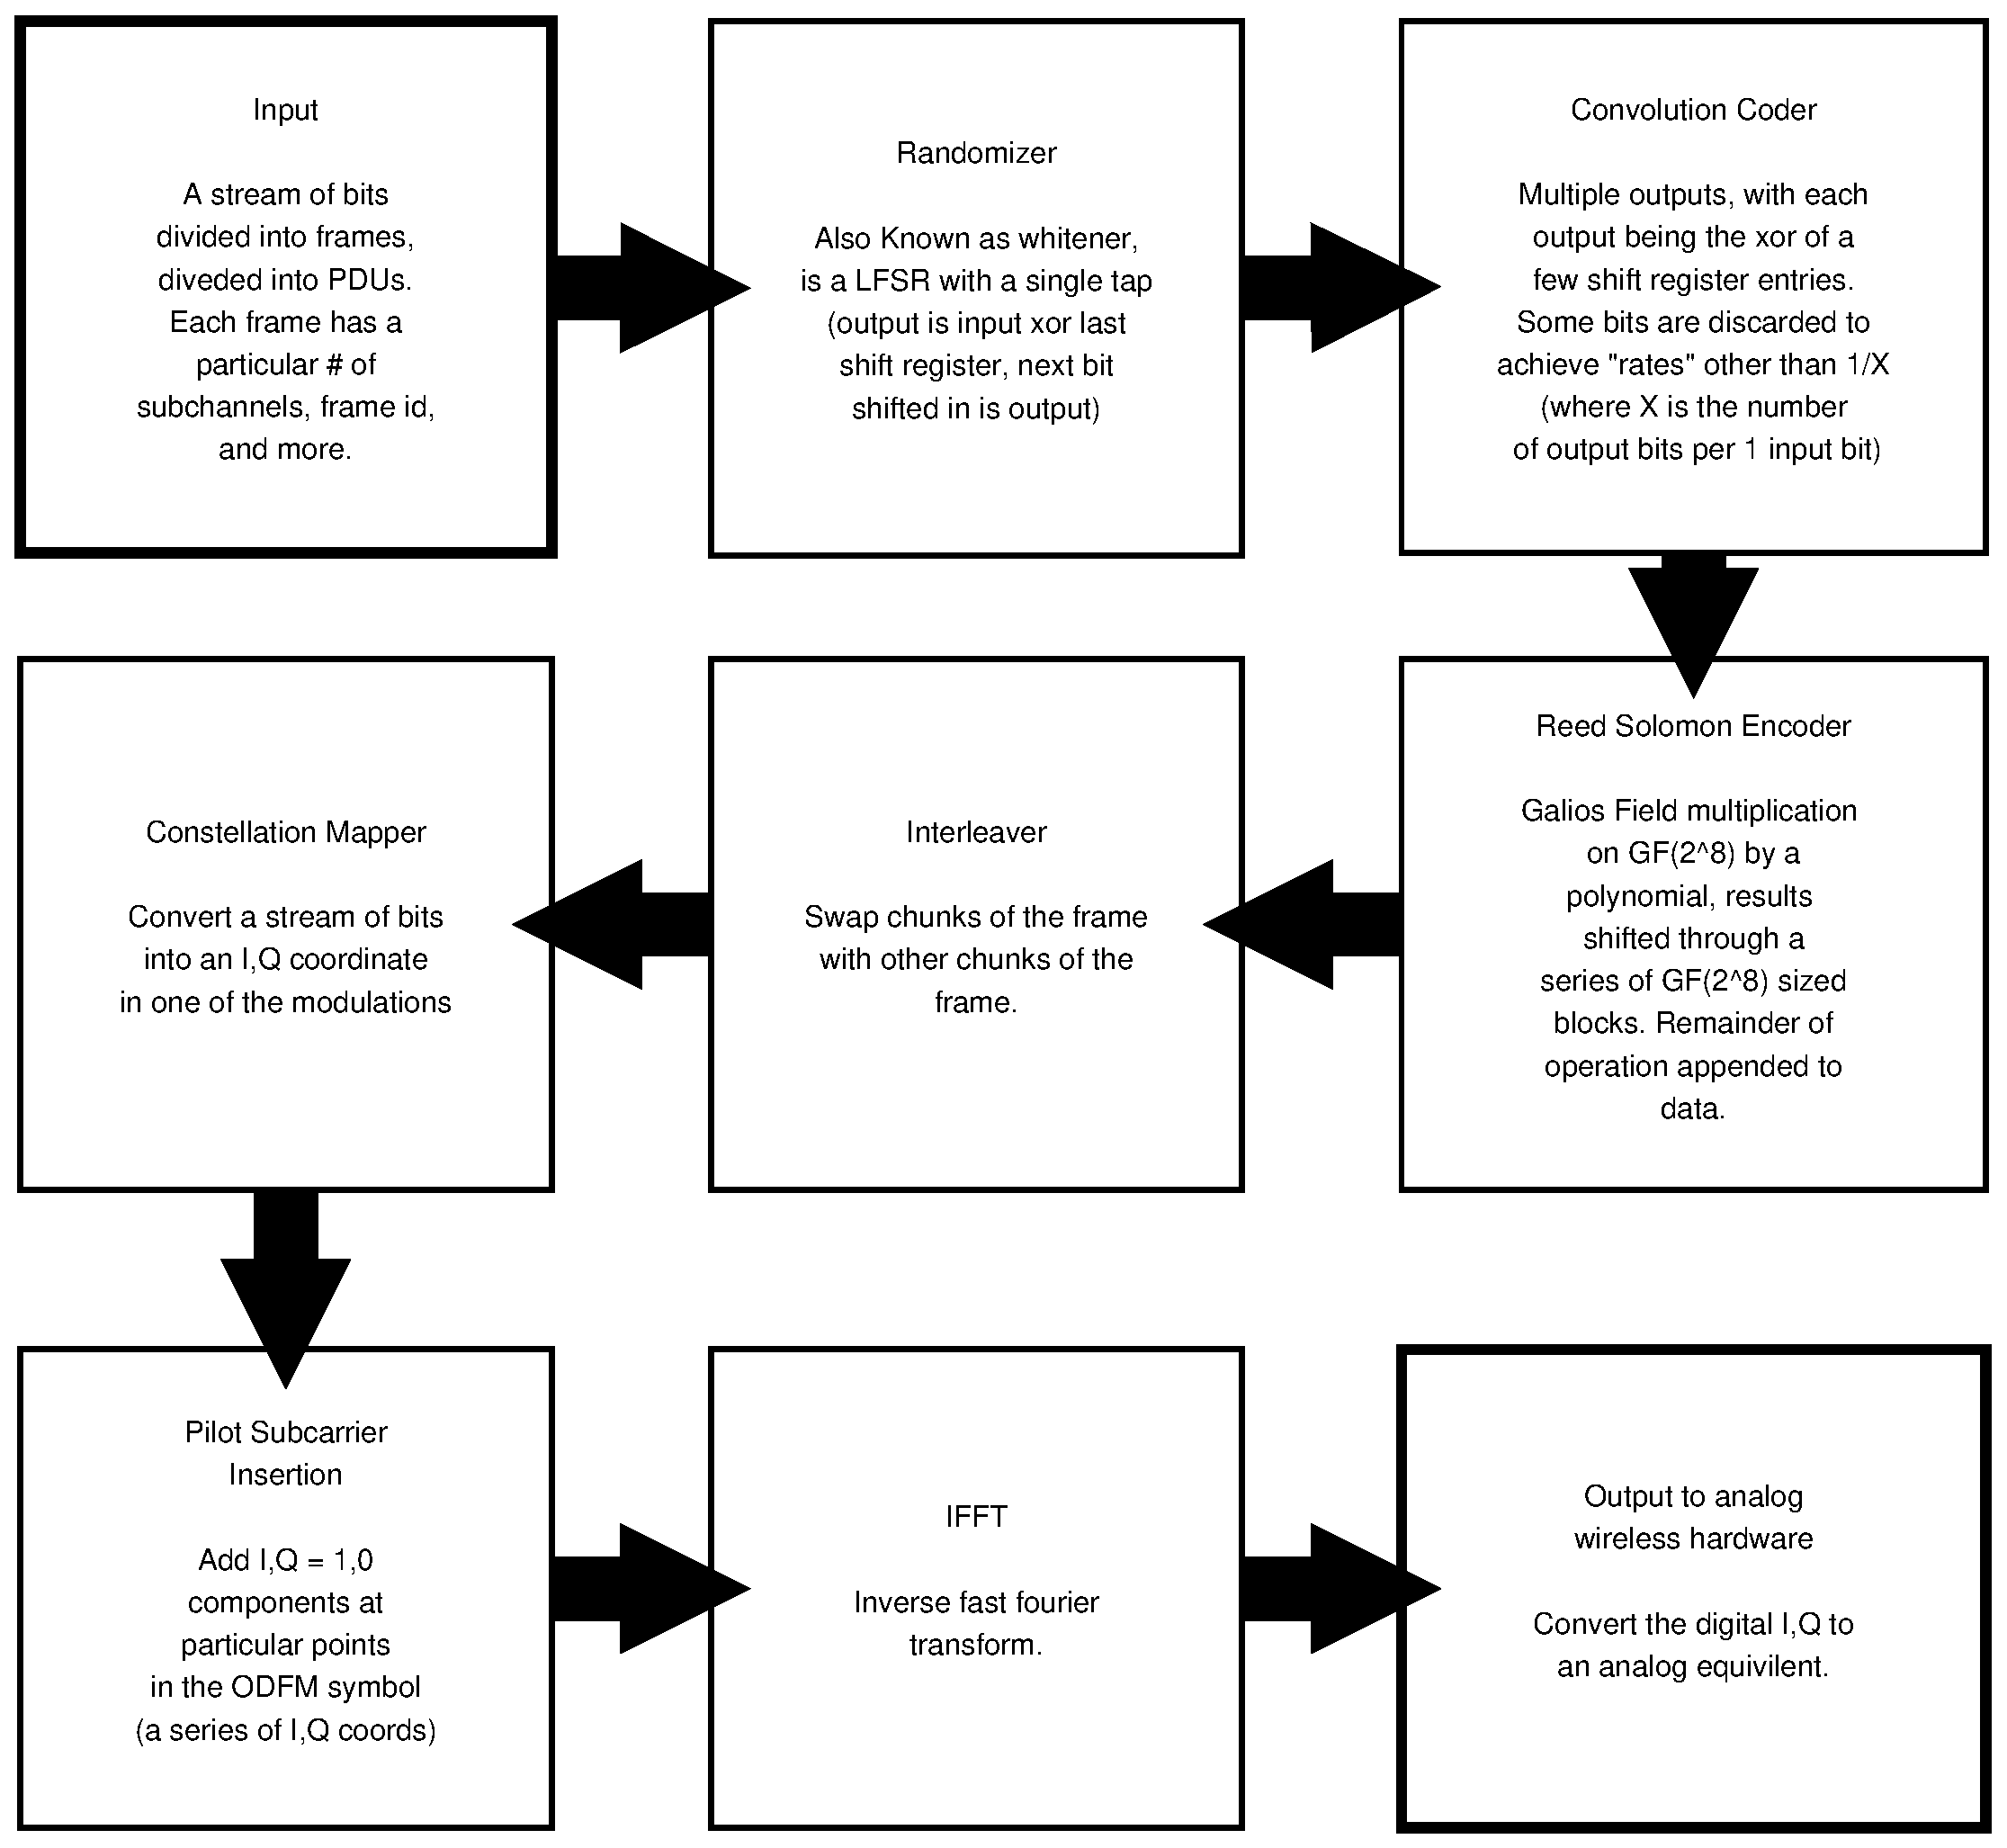
\includegraphics[width=\linewidth]{flow_basic}
		\caption{Basic flow of data through the transmitter}
		\label{fig:flow-basic}
	\end{center}
\end{figure}

\begin{table*}
\begin{tabulary}{\linewidth}{c|C|L}
	\label{tbl:internal-common-wire}
	Name & Active Level & Meaning \\ \hline
	
	\wire{*\_valid} & high & Indicate the source outputting the signal
	is also outputting data (clocked via the \wire{phy\_clock}) which
	should be processed by the next item in the chain. \\

	\wire{*\_bits} & high & A serial stream of bits clocked by
	\wire{phy\_clock}. Only valid when the corresponding
	\wire{*\_valid} line is also active. \\

	\wire{*\_flag} & high & Set active for a single clock cycle
	before becoming inactive again.
\end{tabulary}
\caption{Common signals used internally}
\end{table*}

Each block of the transmitter connected via direct wiring (without a
buffer) is given the same clock. Each block reads its inputs on alternating
clock edges such that two adjacent units read and write on different edges.
This is done so that outputted data does not change while being read.


\begin{figure}
	\begin{center}
		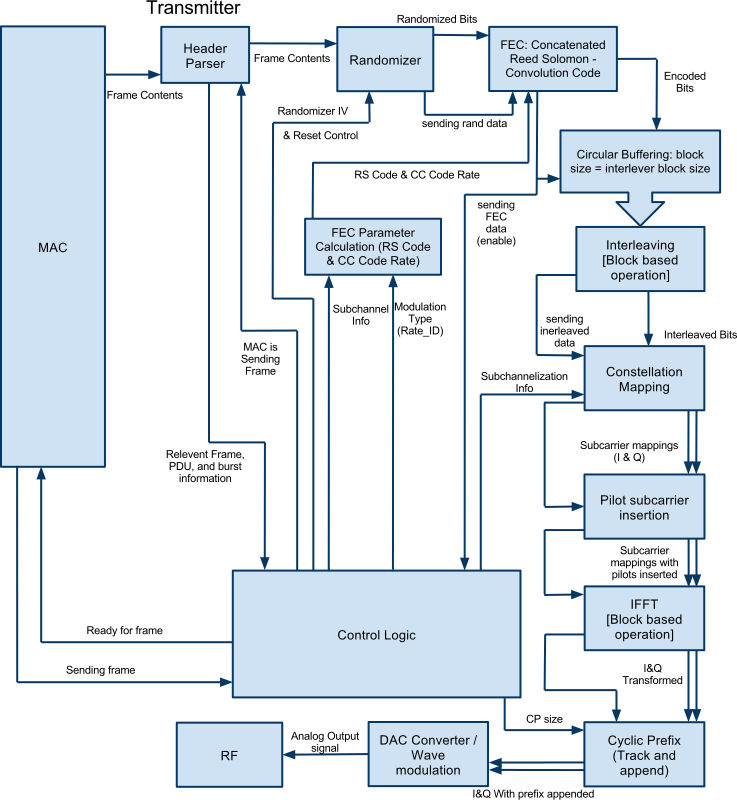
\includegraphics[width=\linewidth]{transmitter}
		\caption{More detailed diagram of the transmitter}
		\label{fig:flow-2}
	\end{center}
\end{figure}


% Actually done
\section{Implimented Modules}

\subsection{Randomizer}
\label{sec:rand}
\begin{description}
	\item[Estimated gates] 1000
	\item[Estimated data bitstream delay] 8 clock cycles for a bit to be
		processed, could be cut to zero by bypassing.
\end{description}

\begin{wrapfigure}{r}{0.5\textwidth}
\begin{center}
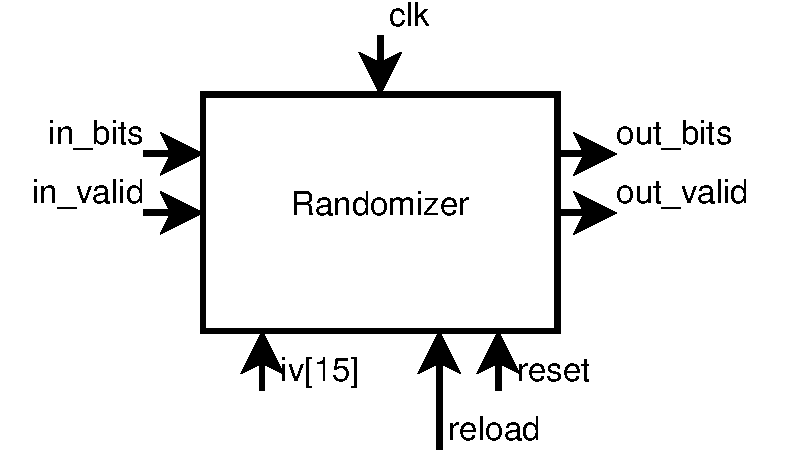
\includegraphics[width=0.48\textwidth]{rand}
\caption{randomizer block diagram}
\label{fig:rand-block}
\end{center}
\end{wrapfigure}

The randomizer operates as a shift register with an initial value
determined by the PDU (packet data unit, one half of a frame) header
and whether it is a UL (uplink) or DL (downlink) PDU.

Internally, the randomizer is implemented as a shift register with a single feedback. 
\autoref{tbl:rand-io} describes the inputs and outputs of the
randomizer. \autoref{fig:rand-block} shows the block representation of the randomizer.

\begin{table*} \begin{tabularx}{\linewidth}{c|c|c|X}
	\label{tbl:rand-io}
	Name & Width & Direction & Description \\ \hline
	
	\wire{reset}     & 1  & I & Resets all internal state
	immediately. The internal register is loaded from
	\wire{iv}. Active low. \\

	\wire{clk}       & 1  & I & Clock. \\

	\wire{in\_bits}  & 1  & I & Uncoded input bitstream to the
	randomizer (this is the first step in the encoding process).\\

	\wire{in\_valid} & 1  & I & Indicates the input bitstream
	\wire{in\_bits} is valid and should be read. \\

	\wire{out\_bits} & 1  & O & Output bitstream. \\
	
	\wire{out\_valid} & 1  & O & Indicates the output bitstream
	is valid. \\

	\wire{iv}        & 15 & I & Initialization data for the
	internal register. \\

	\wire{reload}    & 1  & I & Indicates the internal
	register should be loaded with \wire{iv}. \\

\end{tabularx}
\caption{Randomizer interface definition.}
\end{table*}	
%% TODO: rewrite to only be reed-solomon?
%% or just accept the FEC labeling.

\subsection{Forward Error Correction}

\label{sec:fec}
\begin{description}
	\item[Estimated gates] 2000
	\item[Estimated data bitstream delay] Slightly more than $frac{N_{cbps}}{2} + 8$
\end{description}

This is a Reed-Solomon and convolution coding combination
which is applied per frame. Within the standard, different
RS (Reed-Solomon) codes and CC (convolution code) rates are
used for varying modulation types. As we have fixed the
modulation and code rate to QPSK-1/2, one two of the RS
code and CC rate pairs are needed, as indicated in the
\autoref{tbl:fec-param}.

See \autoref{tbl:fec-io} for a listing of the inputs and outputs.

\subsubsection{Notes on delay}

Both the Reed-Solomon and convolution encoding append additional bits to the bitstream. The convolution encoder emits at most 2 bits for every one bit of input (the 1/2 rate, used with BPSK). The Reed-Solomon encoder appends the residue of its operation to the tail of the bitstream. As it operates of $GF(8)$, 8 bits will be appended. Additionally, between the RS and CC additional bits are appended to such that the bitstream is kept at a multiple of $N_{cbps}$ bytes.

\begin{table*}
	\begin{tabularx}{\linewidth}{X|X|X|X|X|X}
	\label{tbl:fec-param}
		Modulation & Uncoded block size (bytes) &
		Coded block size (bytes) & Overall coding
		rate & RS code & CC code rate \\ \hline
		QPSK & 24 & 48 & 1/2 & (32,24,4) & 2/3 \\
	\end{tabularx}
	\caption{Forward Error correction rates}
\end{table*}

\begin{table*} \begin{tabularx}{\linewidth}{c|c|c|X}
	\label{tbl:fec-io}
	Name & Width & Direction & Description \\ \hline

	\wire{reset} & 1 & I & Active low, resets logic block to initial
	state. \\

	\wire{clk}   & 1 & I & Clocking. \\

	\wire{in\_bits} & 1 & I & Input bitstream, processed by randomizer.
	\\

	\wire{in\_valid} & 1 & I & Indicates the input bitstream
	\wire{in\_bits} should be read.\\

	\wire{out\_bits} & 1 & O & Output bitstream, has FEC
	applied. Will be longer than input bitstream. \\

	\wire{out\_valid} & 1 & O & Indicates the output bitstream
	is valid (the data on it should be read and processed) \\

	\wire{rate\_id} & 3 & I & The type of modulation used. See
	\autoref{tbl:rate-id} for possible values.

\end{tabularx} \caption{FEC interface description} \end{table*}


\subsection{FEC to Interleaver buffer}
\label{sec:fec_buffer}
\begin{description}
	\item[Estimated gates] 1000
	\item[Estimated data bitstream delay] None, all delay is included in the calculation for the Interleaver itself.
\end{description}

\begin{table*} \begin{tabularx}{\linewidth}{c|c|c|X}

	Name & Width & Direction & Description \\ \hline

	\wire{reset} & 1 & I & Active low reset. \\

	\wire{clk} & 1 & I & Clock. \\

	\wire{fec\_out\_bits} & 1 & I & The bitstream outputed by the
	forward error correction unit. \\

	\wire{fec\_out\_valid} & 1 & I & Indicates the bitstream
	\wire{fec\_out\_bits} is valid and should be buffered. \\


	\wire{block} & 768 & O & A block of buffered data. (768 bits = 96
	bytes). \\

	\wire{block\_valid} & 1 & O & Indicates the data block
	\wire{block} is valid and should be processed. \\

	\wire{advance} & 1 & I & Asserted by the consumer to indicate that
	the current data block has been processed completely and a new data
	block is required. \\

\end{tabularx} \caption{FEC output buffer description} 	\label{tbl:fec-buf-io} \end{table*}

\autoref{tbl:fec-buf-io} describes the inputs and outputs of this logic
block.
Transitions the data pipline from a sequence of bits to a sequence of
blocks.

\subsection{Interleaver}
\label{sec:interleaver}
\begin{description}
	\item[Estimated gates] 2000
	\item[Estimated data bitstream delay] About 392 clocks.
\end{description}
	
\begin{table*}
	\begin{tabularx}{\linewidth}{c|c|c|X}
		\label{tbl:interleaver-io}
		Name & Width & Direction & Description \\ \hline
		\wire{reset} & 1 & I & resets the device state. \\
		\wire{clk}   & 1 & I & clocking. \\
		\wire{in\_blk} & 384 & I & Block of input data. \\
		\wire{in\_blk\_valid} & 1 & I & Indicates a block of input data on \wire{in\_blk} is valid and should be processed. \\
		\wire{rate\_id} & 3 & I & The modulation type. Possible values can be found in \autoref{tbl:rate-id}. \\
		\wire{subchan\_ct} & 3 & I & Indicates whether the number of subchannels is 1, 2, 4, 8, or 16. These are paired with values 0, 1, 2, 3, and 4, 
			respectively. The result of other values is undefined. This input allows determintion on how many bits in \wire{in\_blk} should be processed. \\
		\wire{out\_blk} & 384 & O & Interleaved block which is then outputted. \\
		\wire{out\_blk\_valid} & 1 & O & When high, indicates that \wire{out\_blk} contains valid data which should be processed by the next item in the pipeline. 
\end{tabularx} \caption{Interleaver I/O description} \end{table*}

\begin{table*}
	\begin{tabularx}{\linewidth}{X|X|X|X|X|X}
		Subchannels & 16 & 8 & 4 & 2 & 1 \\ \hline
		BPSK   & 192  & 96  & 48  & 24  & 12 \\
		QPSK   & 384  & 192 & 96  & 48  & 24 \\
		16-QAM & 768  & 384 & 192 & 96  & 48 \\
		64-QAM & 1152 & 576 & 288 & 144 & 72
	\end{tabularx} 
	\caption{Values of $N_{cbps}$. Note
	that other than the values listed for QPSK, none of these items are
	supported by this device.}
	\label{tbl:Ncbps}
\end{table*}

All encoded data bits will be interleaved by this block interleaver. The
block size is defined by the number of coded bits per allocated subchannels 
per OFDM symbol ($N_{cbps}$). $N_{cbps}$ is determined by a
combination of the number of subchannels and the modulation used, see
\autoref{tbl:Ncbps} for a listing of possible values.

Interleaving is a two step type operation. The first step ensures adjacent 
coded bits are mapped onto nonadjacent subcarriers and the second step 
ensures bits are mapped alternately onto less and more significant bits of
the constellation. The second step is done to avoid long runs of lowly
reliable bits.
 
The permutations are dependent on the number of coded bits per subcarrier
($N_{cpc}$), which is defined by the type of modulation and the index of the
coded bit before permutation (k).

For our implementation, as we are only using QPSK modulation,
$N_{cpc} = 2$.

k : index of coded bit before first permutation

$m_{k}$ : index after first permutation

$j_{k}$ : index after second permutation 

First permutation equation :
\begin{equation}
m_k = (N_{cbps}/12)*k_{mod12}+floor(k/12)
\end{equation}

Second permutation equation :
\begin{equation}
s=ceil(N_{cpc}/2)
\end{equation}

\begin{eqnarray}
j_k = s*floor(m_{k}/s)+(m_{k}+N_{cbps}- \nonumber \\
	floor(12*m_k/N_{cbps}))_{mod(s)}
\end{eqnarray}

After the interleaving the first bit out of the interleaver would map to the
MSB for the constellation mapping. 

	\subsubsection{Testing and Verification}
	The Interleaver operation can be verified by inputting a known block
	of bits and observing the output. The standard document provides a few of these for our use.

	The verilog code for this module was generated via a python script which directly impliments the permutation equations (\autoref{lst:interleave-gen}). Additionally, a partial non-generated implimentation was created, the equations for which are verified by the same script which generates interleaver code.

	\subsubsection{Implimentation Notes}

Due to the complexity of the permutation, code was written which generates the verilog implimentation for all posible variations in $N_{cpc}$. In a further iteration of the transmitter, a multiplexer would be used to switch to the appropriate interleaver for each type of modulation. A partial implimentation of this multiplexing was written.

The interleaving operation is such that bits much later in the bitstream a swaped with those much earlier in the bitstream. Due to this, the entire OFDM symbol ($N_{cbps}$ bits) must be read into the module prior to a single 1 clock operation to swap the bytes as required. This leads to a rather high cost in delay for this module. % Broken.

% Planned but incomplete.
\section{Planned Modules}

% CONSTELLATION MAPPING

\subsection{Constellation Mapping}
\label{sec:constellation}

\begin{description}
	\item[Estimated gates] 4000
	\item[Estimated data bitstream delay] $N_{cpc}$, the number of bits per constellation. 4 in the case of QPSK.
\end{description}

\begin{table*}
	\begin{tabularx}{\linewidth}{c|c|c|X}

		Name & Width & Direction & Description \\ \hline

		\wire{reset} & 1 & I & When low, the chip is reset. When high, normal operation. \\

		\wire{clk}   & 1 & I & Clocks all synchronous operations. \\

		\wire{in\_bits} & 1 & I & The input bitstream. \\
		\wire{in\_valid} & 1 & I & Indicates that \wire{in\_bits} is valid and should be read. \\
		\wire{out\_Q} & 16 & O & output of Q's. Represents an analog value \\
		\wire{out\_I} & 16 & O & output of I's. Represents an analog value \\
		\wire{out\_valid} & 1 & O & Indicates both \wire{out\_Q} and \wire{out\_I} are valid and should be processed or buffered immediately. \\
		\wire{subchan\_data} & 6 & I & Indicates the mapping of subchannels, see \autoref{tbl:subchan} for explanation of values.
	\end{tabularx}
	\caption{Constellation Mapping input output description}
	\label{tbl:mapping-io}
\end{table*}

The Constellation mapping module takes our bitstream and converts it to a form for an analog radio transmitter. $I$ is used to control the `real' portion of the final output signal while $Q$ controls the `imaginary' component. By placing the $Q$ and $I$ as axis in a 2 dimensional grid, outputs of particular positions are taken to represent particular binary numbers. In BPSK, only 2 outputs are possible, thus the number of bits in the constellation (a particular set of positions on the 2 dimensional grid) is 2. For QPSK, the number of bits per constellation is 4. For this reason, the constellation mapper needs to wait for enough bits to accumulate before it can output 
See \autoref{tbl:mapping-io} for the description of inputs and outputs.


% PILOT INSERTION.

\subsection{Pilot Sub-carrier Insertion}
\label{sec:pilot}
\begin{description}
	\item[Estimated gates] 1000
	\item[Estimated data bitstream delay] UNKNOWN -- FIXME.
\end{description}

Input is (I,Q) pair, output is (I,Q) pair with pilot subcarriers
inserted at some points (fixed).



% IFFT INPUT BUFFER.

\subsection{Sub-carrier to IFFT Buffer}
\label{sec:ifft-buffer}
\begin{description}
	\item[Estimated gates] 2000
	\item[Estimated data bitstream delay] UNKNOWN -- FIXME.
\end{description}
Insertion into this buffer is ordered but will have random
jumps around different UL \& DL bursts.

Block Size = blk\_siz = 200 (the total number of used
subcarriers)

Buffers blk\_size items each of which has width 2 bits.
QPSK utilizes both I and Q, amplitude and phase, each with
a granularity of 2. This means that each item (a pair of I
\& Q) has 4 possible values and thus 2 bits are needed for
each.

%\todo[inline]{Pilot insertion input needs to be defined}
\begin{table*}\begin{tabularx}{\linewidth}{c|c|c|X}
	\label{tbl:ifft-buffer-io}
			
	Name & Width & Direction & Description \\ \hline

	\wire{reset} & 1 & I & Resets the device state. \\

	\wire{clk}   & 1 & I & Clocking. \\

	\wire{in\_blk} & $??$ & I & Input data from the Pilot Insertion. \\

	\wire{in\_blk\_valid} & 1 & I & When high, indicates that the input block is
	valid and should be processed. \\

	\wire{out\_blk} & $200 \cdot 2 \cdot 16$ & O & Output data to the IFFT. Width of
	numbers is 16 bits, processing both Q and I. \\

	\wire{out\_blk\_valid} & 1 & O & Indicates the output block
	\wire{out\_blk} is valid and should be imediately copied (it will be
	replaced by the next block on the next clock cycle).

\end{tabularx}
\caption{Sub-carrier to IFFT Buffer input/output description.}
\end{table*}


% IFFT

\subsection{IFFT}
\label{sec:ifft}
\begin{description}
	\item[Estimated gates] 10,000
	\item[Estimated data bitstream delay] UNKNOWN -- FIXME.
\end{description}

The IFFT must process 256 complex numbers with a depth of 16 bits for each
component (16 bits for the Real component and an another 16 bits for the
imaginary).

See \autoref{tbl:ifft-io} for a description of the inputs and outputs.
	
	Buffers blk\_size items each of which has width 2 bits.
	QPSK utilizes both I and Q, amplitude and phase, each with
	a granularity of 2. This means that each item (a pair of I
	\& Q) has 4 possible values and thus 2 bits are needed for
	each.

	The IFFT takes in 256-bit complex samples and outputs to the Cyclic Prefix.

\begin{table*}
	\begin{tabularx}{\linewidth}{c|c|c|X}
		\label{tbl:ifft-io}
			
	Name & Width & Direction & Description \\ \hline

	\wire{reset} & 1 & I & Resets the device state. \\

	\wire{clk}   & 1 & I & Clocking. \\

	\wire{in\_blk\_valid} & 1 & I & When high, indicates that the input block is
	valid and should be processed. \\

	\wire{in\_blk} & $200 \cdot 2 \cdot 16$ & I & Input data for the IFFT. Width of
	numbers is 16 bits, processing both Q and I. \\

	\wire{out\_blk} & $256 \cdot 2 \cdot 16$ & O & Output data after IFFT is preformed. Width of
	numbers is 16 bits, processing both Q and I. \\

	\wire{out\_blk\_valid} & 1 & O & Indicates the output block
	\wire{out\_blk} is valid and should be imediately copied (it will be
	replaced by the next block on the next clock cycle).

\end{tabularx}
\caption{IFFT input/output description.}
\end{table*}
%% CYCLIC PRERIX


\subsection{Cyclic Prefix}
\label{sec:cyclic_prefix}
\begin{description}
	\item[Estimated gates] 2000
	\item[Estimated data bitstream delay] About 1050 clocks.
\end{description}

The Cyclic Prefix is used to act as protection from Intersymbol Interference 
by duplicating a certain number of symbols defined by the $CP_rate$.

The Cyclic Prefix appends to the front of the symbol a copy of the last
$256/CP_{rate}$ ($N_{IFFT}/CP_{rate}$) bits. OFDM PHY should allow for four
(4) rates as defined by 2 bits in the PHY Mode ID field. 

It reads 256 2 bit items from the IFFT into 2 256 blocks of memory.
On output, the appropriate number of bits are read from the end of 
memory by offset.

At a rate of $1/4$, 64 bits would need to be read from the end and 
at a rate of $1/32$, 8 bits would need to be read.

The sample size would then increase from 256 bits to anywhere between
264 to 320 bits.

For our implementation, we will set the CP rate at $1/16$ which leads to
a sample size of 272 bits.

This process would take about about 512 clocks to read in the data to fill
memory and about 528 clocks to write out. 

The total time would include clocks to set and check valid lines and would
total to about 1050 clocks. 

\begin{table}
	\begin{tabulary}{\linewidth}{C|C}
		Value of \wire{param\_G} & Ratio of CP time to ``useful'' time. \\ \hline
		0b00 & 1/4 \\
		0b01 & 1/8 \\
		0b10 & 1/16 \\
		0b11 & 1/32
	\end{tabulary}
	\caption{Values of OFDM parameter G as presented on \wire{param\_G}}
	\label{tbl:param-g-vals}
\end{table}

\begin{table*}
	\begin{tabularx}{\linewidth}{c|c|c|X}
		Name & Direction & Width & Description \\ \hline
		\wire{param\_G} & I & 2 & The meanings of valid values
		are listed in \autoref{tbl:param-g-vals}. Indicates the
		fraction of CP time to ``useful'' time. \\
		\wire{cp\_in\_bits} & I & 1 & Input bitstream. \\
		\wire{cp\_in\_valid} & I & 1 & Indicates the input bitstream \wire{cp\_in\_bits} is valid. \\
		\wire{cp\_out\_bits} & O & 1 & Output bitstream. \\
		\wire{cp\_out\_valid} & O & 1 & Indicates the output bitstream \wire{cp\_out\_bits} is valid.
	\end{tabularx}
	\caption{Cyclic Prefix Inputs and Outputs}
	\label{tbl:cp-io}	
\end{table*}

\autoref{tbl:cp-io} lists the inputs and outputs to the cyclic
prefix unit.

Appends the last Tg items of the previous frame to the start of the
present frame.  Reads 256 by 2 16 bit items from the IFFT, appending Tg
items to the start of it. It also stores the last Tg items so that
they may be appended to the next frame from the IFFT.

%\comment{\todo[inline]{Maximum Size needed?}}
 % Broken.

%% FRAME

\subsection{Frame Handler}
\begin{description}
	\item[Estimated gates] 2000
	\item[Estimated bitstream delay] 2 clock cycles for a bit to be
		processed 
\end{description}

Is given a bitstream directly from the MAC device, expected to be able to
clock in this bit stream at the rate defined by the MAC. Data and
parsed configuration is sent to the Burst Handler (\autoref{sec:burst})
to be processed and outputed.

Inputs and outputs are listed in \autoref{tbl:frame-io}.

\begin{table} \begin{center} \begin{tabularx}{\linewidth}{c|c}
	\label{tbl:rate-id}
	\wire{rate\_id[3]} & Modulation RS-CC rate \\ \hline
	0 & BPSK-1/2 \\
	1 & QPSK-1/2 \\
	2 & QPSK-3/4 \\
	3 & 16-QAM-1/2 \\
	4 & 16-QAM-3/4 \\
	5 & 64-QAM-2/3 \\
	6 & 64-QAM-3/4 \\
	7 & Reserved
\end{tabularx} \caption{Possible values for \wire{rate\_id}. Note that
All values but 1 (QPSK-1/2) are unsupported by this device.}
\end{center} \end{table}

\begin{table*}
	\label{tbl:subchan}
	
	\caption{Possible values for \wire{subchan\_data}.}
\end{table*}

\begin{table*} \begin{tabularx}{\linewidth}{c|c|c|X} \label{tbl:frame-io}
	Name & Width & Direction & Description \\ \hline

	\wire{clk} & 1 & I & Clocks the logic block.\\

	\wire{reset} & 1 & I & Active low reset to initial state. \\


	\wire{frame\_in\_bits} & 1 & I & Input bitstream, clocked via
	\wire{frame\_in\_clk}. \\

	\wire{frame\_in\_clk} & 1 & I & Positive edge indicates that data on
	\wire{frame\_in\_bits} should be read. \\
	
	\wire{frame\_in\_valid} & 1 & I & Set high while the current series
	of bits is part of the same frame. \\

	\wire{burst\_reset} & 1 & O & reset line to the burst handler
	(\autoref{sec:burst}). \\

	\wire{burst\_bits} & 1 & O & Bits to the burst handler. \\

	\wire{burst\_valid} & 1 & O & indicates the bitstream
	\wire{burst\_bits} is valid and should be processed. \\


	\wire{frame\_num} & 4 & O & The frame number parsed from the header
	structures. \\

	\wire{iuc} & 4 & O & The UIUC or DIUC field, parsed from the header
	stuctures. Only valid for the currently outputed burst. \\

	\wire{subchan\_data} & 6 & O & See \autoref{tbl:frame-io}.
	\autoref{tbl:subchan} describes valid values. Per burst. \\

	\wire{rate\_id} & 3 & O & See \autoref{tbl:rate-id}. Per burst. \\

\end{tabularx} \caption{Frame Handler interface description} \end{table*}

%% BURST

\subsection{Burst Handler} \label{sec:burst}
\begin{description}
	\item[Estimated gates] 2000 
	\item[Estimated data bitstream delay] 2 clock cycles for a bit to be
		processed, could be cut to zero by bypassing.
\end{description}

Bursts are composed of multiple OFDM symbols. OFDM symbols are composed of
multiple sub-channels.\autoref{tbl:burst-io} shows the burst interface inputs and outputs.
Across a single burst initialization of the pipeline hardware will not
change.

\begin{table*} \begin{tabularx}{\linewidth}{c|c|c|X}
	\label{tbl:burst-io}
	Name & Width & Direction & Description \\ \hline
	
	\wire{reset} & 1 & I & Imediately resets the burst handler. Active
	low. \\

	\wire{clk} & 1 & I & Clocking. \\

	\wire{iuc} & 4 & I & The UIUC or DIUC field (depending on uplink
	or downlink state). Used by randomizer. \\
	
	\wire{bsid} & 4 & I & Used by randomizer. \\
	
	\wire{frame\_num} & 4 & I & Used by randomizer. \\

	\wire{burst\_in\_bits} & 1 & I & Input bitstream. \\

	\wire{burst\_in\_valid} & 1 &  I & Indicates the input bitstream
	\wire{burst\_in\_bits} is valid. \\

	\wire{rand\_iv} & 15 & O & The initialization for
	the randomizer's internal register. \\

	\wire{rand\_reload} & 1 & O & Instructs the randomizer to reload
	it's internal register with a new one outputed on
	\wire{rand\_iv}. \\

	\wire{burst\_out\_bits} & 1 & O & Output bitstream. Sent to the
	randomizer for first portion of processing. \\

	\wire{burst\_out\_valid} & 1 & O & Indicates output is valid.
	Also attached to the randomizer. \\

	\wire{subchan\_data\_in} & 6 & I & See \autoref{tbl:frame-io}.
	\autoref{tbl:subchan} describes valid values. \\

	\wire{subchan\_data\_out} & 6 & O & Output pair of
	\wire{subchan\_data\_in}, simple pass through. \\

	\wire{subchan\_ct} & 4 & O & Indicates the number of subchannels in
	use. Calculated from \wire{subchan\_data\_in}. \\

	\wire{rate\_id\_in} & 3 & I  & See \autoref{tbl:rate-id}. \\

	\wire{rate\_id\_out} & 3 & O & Pass-through pair of
	\wire{rate\_id\_in}. \\

\end{tabularx}
\caption{Interface definition for the Burst Handler.}
\end{table*}




% Required in example.
\section{Health, Safety, and Environmental Issues}

\subsection{Product Dangers}

Potential for heat, radiation, and distraction while operating equipment (depending on what type of end-user device this implementation is integrated into. As this is only a component of an arbitrary end user device, dangers caused or directly inferred from its use are limited.

\subsection{Health Hazards}

As a wireless transmitter, certain power outputs at particular frequencies could be dangerous for people to be in close proximity to. These power levels and transmission frequencies are not handled within this project, rather, they fall to the real of the analog transmitter portion.

\subsection{Environmental Hazards}

As a wireless device, any implementation utilizing this code will need to obtain FCC approval to ensure it properly uses the frequency ``space'' allocated to it. Notably, the WiMAX specification provides for both licensed and unlicensed frequency range use, meaning additional approval could be required from the owner of the particular band the device operates in.

% Notes on where improvements could be made.
\section{Conclution}

This design failed to be completed. Reexamining the plan of design for this project reveals a few issues that made effective implimentation difficult. Planning on a lack of delay communication between hardware modules creates a significant amount of planning difficulty. Every module's input and output speed must be able to be predetermined and buffers (which understand how to handle delays) added. This can result in the use of numerous overly large buffers due to worse case calculations being used to determine the buffer size. Additionally, this plan is made more difficult by multple 802.16 frames being pushed through the same hardware one after the other. As the number of outputed bits (prior to conversion to wide Q and I signals) is larger than the number of inputed bits, a delay between frame inputs from outside the system or a buffer of infinite size is required. Clearly, infinite flip-flops are not a posibility in any logic circuit, thus the system as a whole would need an understanding of when it was "ready" for more data.

Further along the same track, the current design does not allow for the use of internal modules for seperate frames simultaniously. For example, the reed-solomon encoder cannot be easily used for one frame while the convolution coder begins processing the next. One possible plan to allow this to be done simplely is to have a signal between modules for when a frame begins or ends (rather than using a central piece of logic to manage this). Unfortunately, we need more than just knowledge of when the frame begins and ends to properly process it; a whole slew of metadata needs to be passed along while being timed properly with the motion of the bitstream through the system. Additionally this metadata would need to handle delays properly (as using solely buffering is unfeasable). From these requirements, the posibilility of using a second bitstream to carry the metadata arises, as shown in \autoref{fig:alt-bitstream}. Each module could stay as intitially designed, but be wrapped in a conrtoller which handles extraction of metadata from the bitstream as well as properly handling it's timing. It could be passed along ahead of the start of a frame such that when the actual data reaches a new module, the necissary metadata for processing it is already present. Of course, additional issues arise if the metadata bitstream can exceed the length of the shortest 802.16 frame: an additional delay would need to be inserted after a short frame to give time for the metadata to be transfered.

Using an FPGA for this is probably not economically viable or efficient. Power consumption would be much higher than could be achieved with a non-FPGA realization. Cost would also be an issue for any product with a non-inconsiquential volume of production. As wireless devices are often  mobile and battery powered, power consumption is a serious concern. Additionally, using this as portion of a larger FPGA design would not be feasable due to the high use of logic circuit resources by various components, primarily the (planned) IFFT.


\begin{figure}
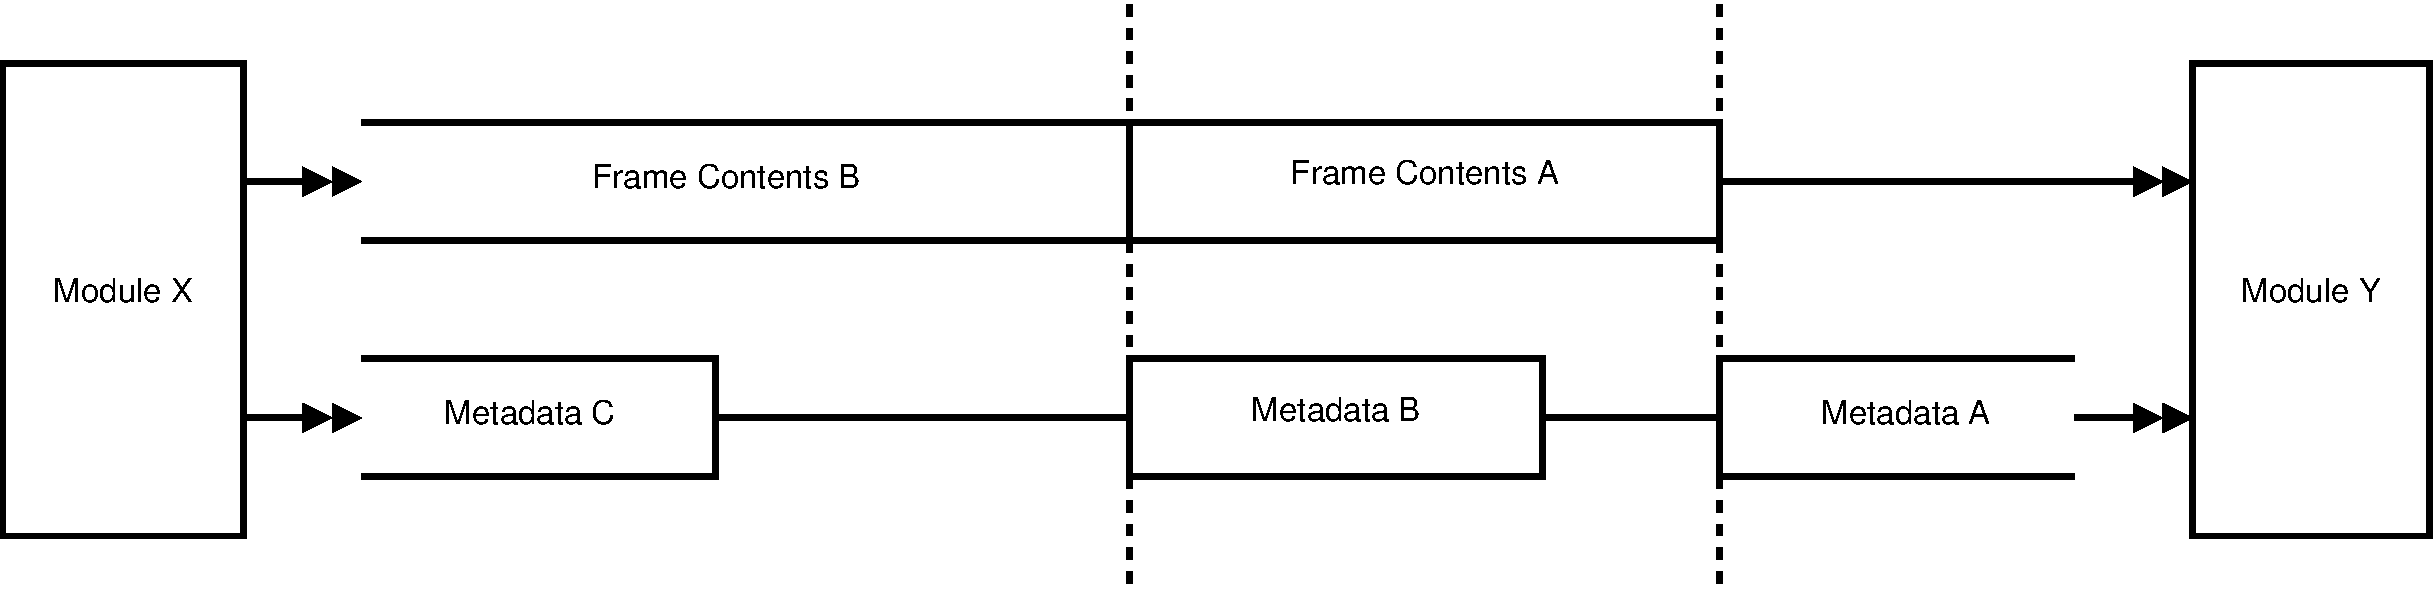
\includegraphics[width=\linewidth]{conclution_metadata_transfer}
\caption{Proposed Bitstream Transfer Pattern	}
\label{fig:alt-bitstream}
\end{figure}


\appendix

% Appendix containing code.
\todo{Appendix with Code}

\bibliography{doc}{}
\bibliographystyle{ieeetr}

\end{document}